\documentclass[tikz,border=2pt]{standalone}

% Pure TikZ; no pgfplots axes needed. The `patterns.meta` library is also
% skipped to keep the compile compatible with minimal TinyTeX installs.
\usetikzlibrary{arrows.meta, positioning, calc, patterns,
                decorations.pathmorphing}

% Colour palette (B&W-safe: each tone pairs with a pattern).
\definecolor{waterFill}{HTML}{e8eef5}
\definecolor{soilFill}{HTML}{e6ddc8}
\definecolor{scourFill}{HTML}{f2e8d8}
\definecolor{steelFill}{HTML}{1a1a1a}
\definecolor{accent}{HTML}{0b3d91}

% ---- Dimensions (prototype scale, metres, 1 cm = 1 m) ---------------------
\def\bucketR{4.0}         % bucket radius (D / 2)
\def\bucketL{9.3}         % skirt penetration
\def\waterD{5.0}          % water column height above mudline
\def\soilBelow{4.0}       % extra soil below tip to draw
\def\scourDepth{2.0}      % example scour depth for annotation (S)
\def\scourHalf{8.0}       % scour-hole half-width at seabed
\def\pageLeft{-12.0}
\def\pageRight{12.0}
\def\lidT{0.35}           % lid drawing thickness (cosmetic)

\begin{document}
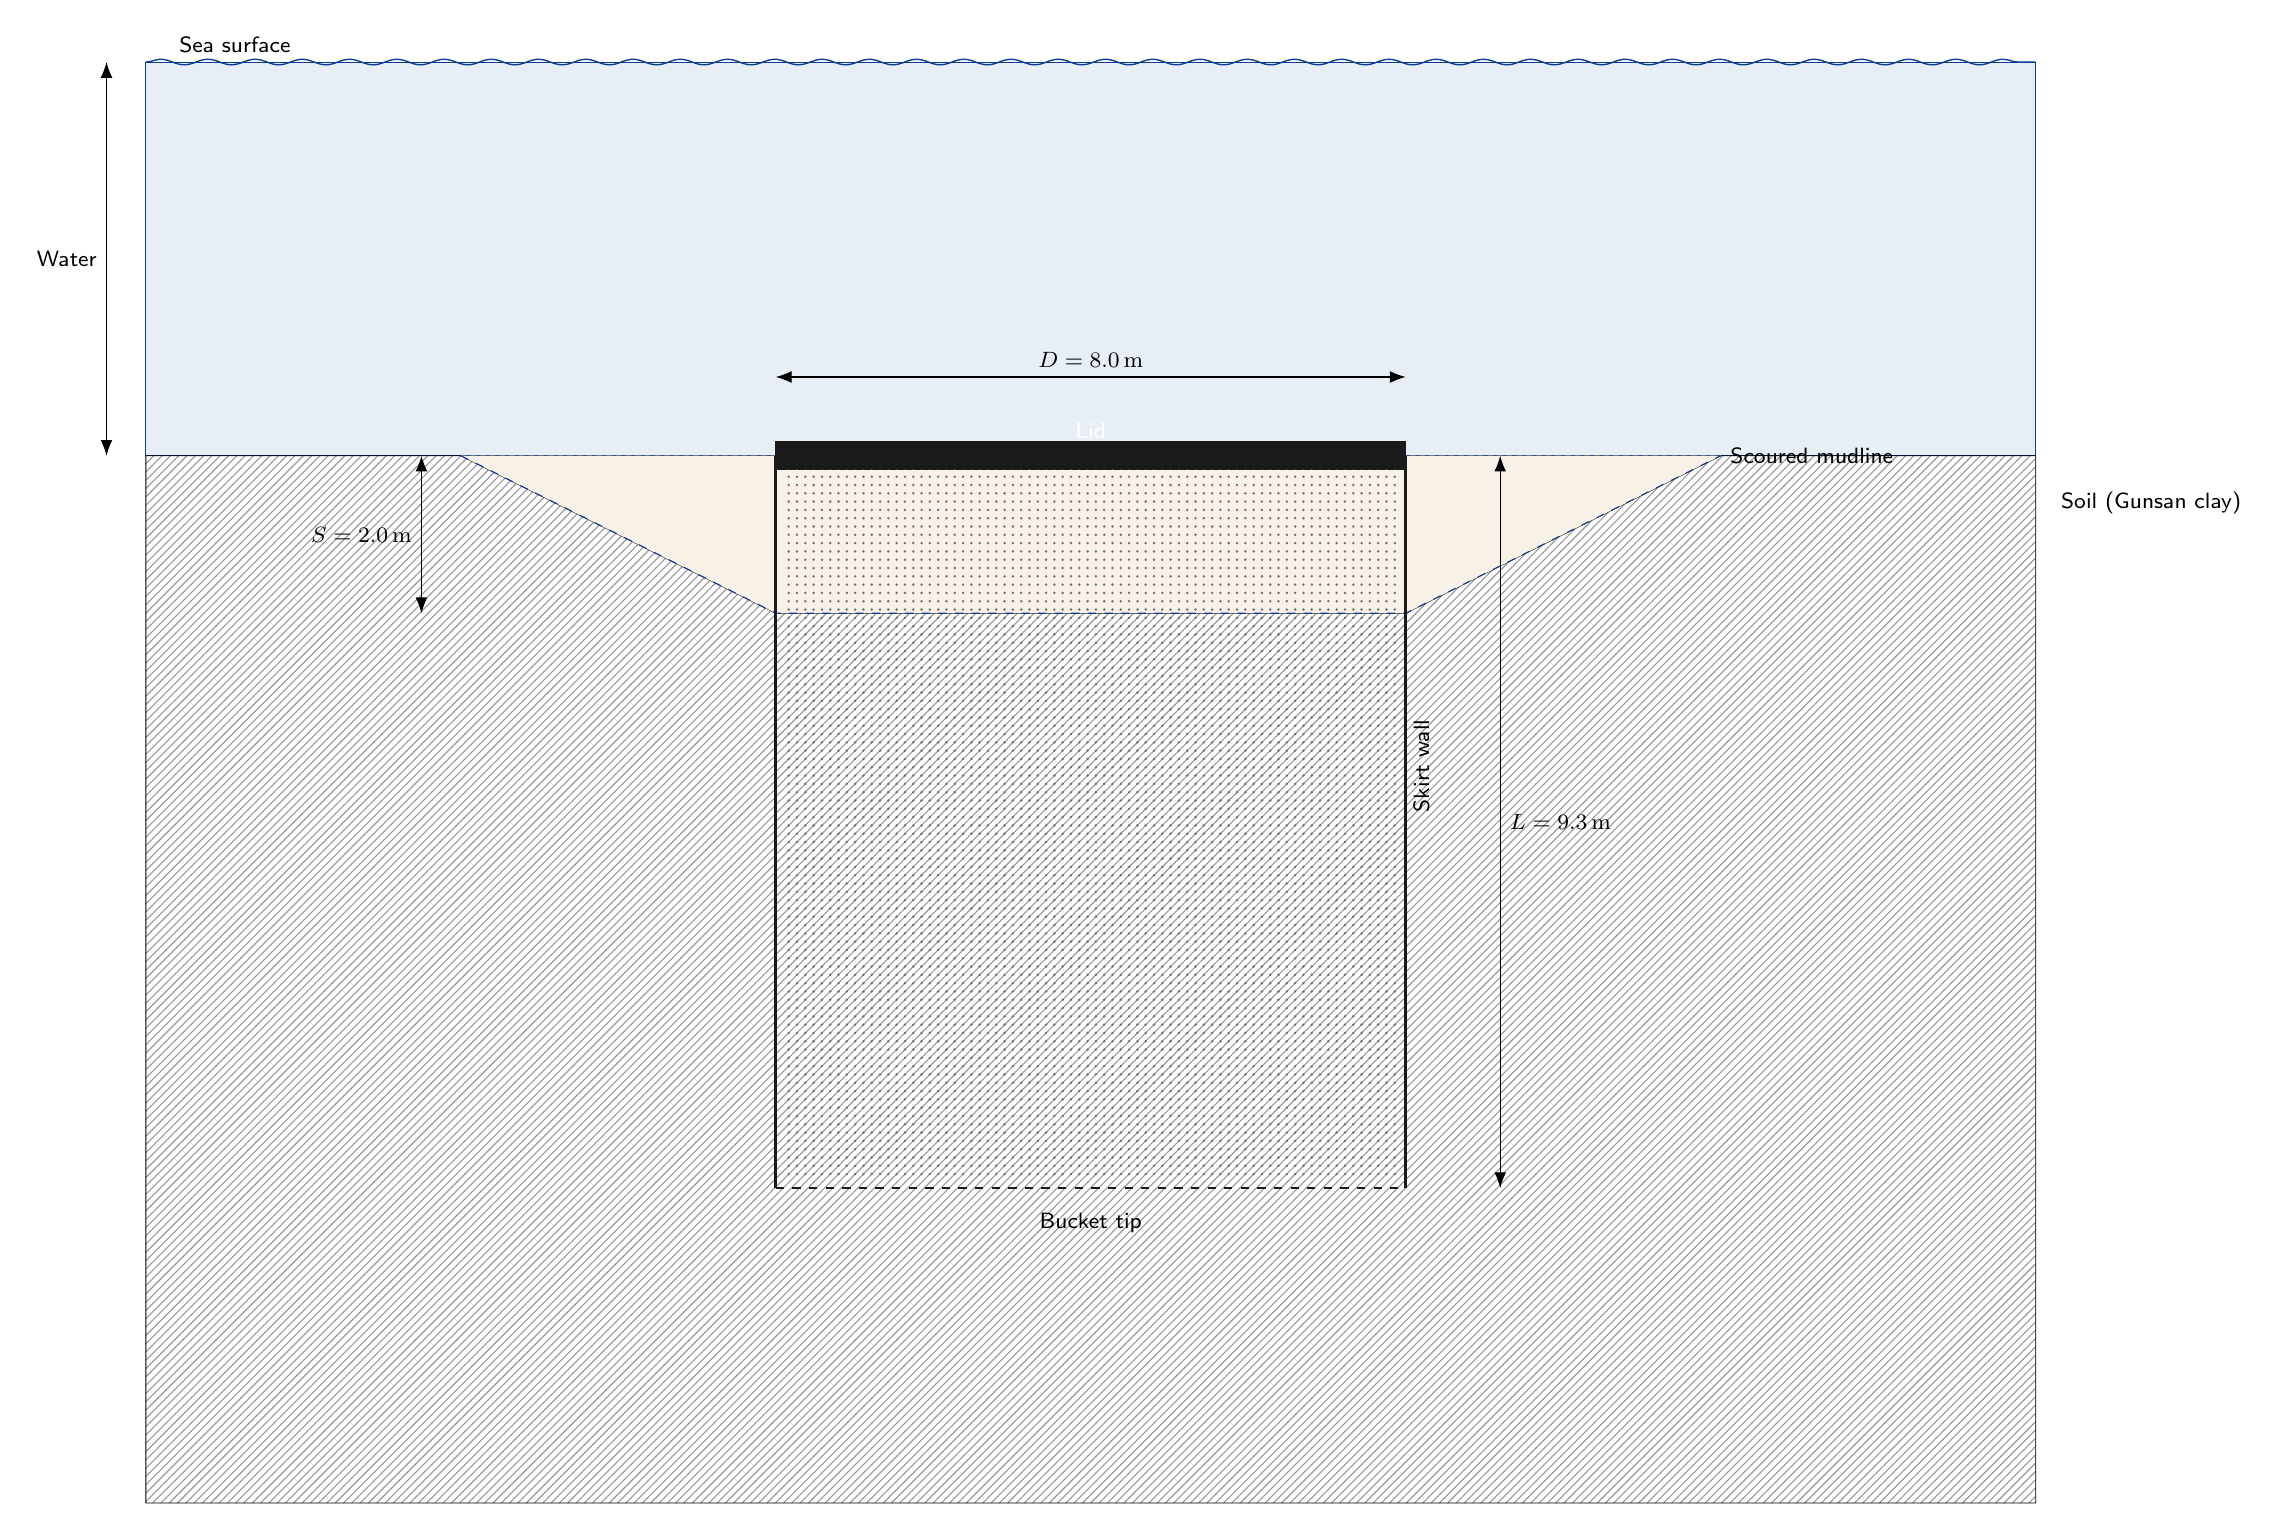
\begin{tikzpicture}[x=1cm, y=1cm,
                    font=\sffamily\small]

    % ==========================================================
    % 1. NAMED COORDINATES (all geometry referenced from here)
    % ==========================================================
    \coordinate (waterTL) at (\pageLeft,  \waterD);
    \coordinate (waterTR) at (\pageRight, \waterD);
    \coordinate (waterBL) at (\pageLeft,  0);
    \coordinate (waterBR) at (\pageRight, 0);

    \coordinate (soilTL)  at (\pageLeft,  0);
    \coordinate (soilTR)  at (\pageRight, 0);
    \coordinate (soilBL)  at (\pageLeft,  -\bucketL-\soilBelow);
    \coordinate (soilBR)  at (\pageRight, -\bucketL-\soilBelow);

    \coordinate (lidL)    at (-\bucketR, 0);
    \coordinate (lidR)    at ( \bucketR, 0);
    \coordinate (tipL)    at (-\bucketR, -\bucketL);
    \coordinate (tipR)    at ( \bucketR, -\bucketL);

    \coordinate (scourL)  at (-\scourHalf, 0);
    \coordinate (scourR)  at ( \scourHalf, 0);
    \coordinate (scourBotL) at (-\bucketR, -\scourDepth);
    \coordinate (scourBotR) at ( \bucketR, -\scourDepth);

    % ==========================================================
    % 2. WATER LAYER
    % ==========================================================
    \filldraw[fill=waterFill, draw=accent, line width=0.3pt]
        (waterBL) -- (waterBR) -- (waterTR) -- (waterTL) -- cycle;
    % Wavy surface
    \draw[accent, line width=0.5pt, decorate,
          decoration={snake, amplitude=1pt, segment length=6mm}]
        (waterTL) -- (waterTR);

    % ==========================================================
    % 3. SOIL LAYER (with scour hole carved out of the top)
    % ==========================================================
    \filldraw[fill=soilFill, draw=black, line width=0.3pt,
              pattern=north east lines, pattern color=black!40]
        (soilBL) -- (soilBR) -- (soilTR)
        -- (scourR) -- (scourBotR) -- (scourBotL) -- (scourL)
        -- (soilTL) -- cycle;

    % ==========================================================
    % 4. SCOUR HOLE FILL (lighter tone so it reads as "no soil here")
    % ==========================================================
    \filldraw[fill=scourFill!60, draw=accent, line width=0.4pt, dashed]
        (scourL) -- (scourBotL) -- (scourBotR) -- (scourR);

    % Original mudline as faint dashed reference
    \draw[black!55, line width=0.3pt, dash pattern=on 2pt off 1.5pt]
        (scourL) -- (scourR);

    % ==========================================================
    % 5. SUCTION BUCKET (skirt + lid)
    % ==========================================================
    % Skirts (two walls)
    \draw[steelFill, line width=1.0pt] (lidL) -- (tipL);
    \draw[steelFill, line width=1.0pt] (lidR) -- (tipR);
    % Bucket tip lip (thin dashed bottom)
    \draw[steelFill, line width=0.5pt, dashed] (tipL) -- (tipR);

    % Lid (dark filled rectangle sitting on top of skirts)
    \filldraw[fill=steelFill, draw=steelFill]
        ($(lidL) + (0, -\lidT/2)$) rectangle ($(lidR) + (0, \lidT/2)$);

    % Soil plug inside bucket (dots pattern to differentiate from hatch)
    \filldraw[fill=soilFill!80, draw=none,
              pattern=dots, pattern color=black!55]
        ($(lidL)+(0.1, -\lidT/2)$)
          rectangle
        ($(tipR)+(-0.1, +0.1)$);

    % ==========================================================
    % 6. DIMENSION ARROWS + LABELS
    % ==========================================================
    % D (bucket diameter) — above the lid, inside water
    \draw[{Latex[length=2mm]}-{Latex[length=2mm]}, line width=0.4pt]
        ($(lidL) + (0, 1.0)$) -- ($(lidR) + (0, 1.0)$)
        node[midway, above, font=\sffamily\footnotesize]
            {$D = 8.0\,\mathrm{m}$};

    % L (skirt length) — on the right side of the bucket, vertical
    \draw[{Latex[length=2mm]}-{Latex[length=2mm]}, line width=0.4pt]
        ($(lidR) + (1.2, 0)$) -- ($(tipR) + (1.2, 0)$)
        node[midway, right, font=\sffamily\footnotesize]
            {$L = 9.3\,\mathrm{m}$};

    % S (scour depth) — inside the scour hole, vertical
    \draw[{Latex[length=2mm]}-{Latex[length=2mm]}, line width=0.4pt]
        ($(scourL) + (-0.5, 0)$) -- ($(scourL) + (-0.5, -\scourDepth)$)
        node[midway, left, font=\sffamily\footnotesize]
            {$S = 2.0\,\mathrm{m}$};

    % Water depth (optional, on the far left)
    \draw[{Latex[length=2mm]}-{Latex[length=2mm]}, line width=0.4pt]
        (waterTL) ++(-0.5, 0) -- ($(waterTL) + (-0.5, -\waterD)$)
        node[midway, left, font=\sffamily\footnotesize]
            {Water};

    % ==========================================================
    % 7. CALLOUT LABELS
    % ==========================================================
    \node[font=\sffamily\footnotesize, anchor=west] at (scourR) {Scoured mudline};
    \node[font=\sffamily\footnotesize, anchor=west] at ($(soilTR) + (0.2, -0.6)$)
        {Soil (Gunsan clay)};
    \node[font=\sffamily\footnotesize, white, anchor=south]
        at ($(lidL)!0.5!(lidR) + (0, 0.1)$) {Lid};
    \node[font=\sffamily\footnotesize, anchor=south west]
        at ($(waterTL) + (0.3, 0.0)$) {Sea surface};
    \node[font=\sffamily\footnotesize, anchor=north]
        at ($(tipL)!0.5!(tipR) + (0, -0.2)$) {Bucket tip};
    \node[font=\sffamily\footnotesize, anchor=west, rotate=90]
        at ($(lidR)!0.5!(tipR) + (0.2, 0.0)$) {Skirt wall};

\end{tikzpicture}
\end{document}
